\Chapter{Learning Efficient Correlated Equlibria: Can agents in a distributed system learn a payoff maximizing correlated equilibrium, despite severely limited information about one another's behavior?}\label{ch3}

%Agents' control laws are a crucial component of any multiagent system. They dictate how individual agents process locally available information to make decisions. Factors that determine the quality of a control law include informational dependencies, asymptotic guarantees, and convergence rates. 

%Game theory has recently emerged as a framework for assigning agents' local control laws in a distributed system \cite{Lasaulce2011,Alpcan2010,Han2012,MacKenzie2006,Menache2011}. Here, a {\it learning rule} dictates how each agent should revise its behavior, based on its individual objective and on available information about the surrounding environment. Significant research has been directed at deriving distributed learning rules that possess desirable asymptotic performance guarantees and convergence rates and enable agents to make decisions based on limited information.

%The majority of this research has focused on attaining convergence to (pure) Nash equilibria under stringent information conditions \cite{Young2009, Frihauf2012, Foster2006, Boussaton2012, Poveda2013, Gharesifard2012}. Recently, the research focus has shifted to ensuring convergence to alternate types of equilibria that often yield more efficient behavior than Nash equilibria.  In particular, results have emerged that guarantee convergence to Pareto efficient Nash equilibria \cite{Marden2009,Pradelski2012}, potential function maximizers \cite{Blume1993, Marden2012}, welfare maximizing action profiles \cite{Marden2011, Arieli2012}, and the set of correlated equilibria \cite{Hart2000,Marden2013c,Aumann1987,Foster1997}, among others.  

%In most cases highlighted above, the derived algorithms guarantee (probabilistic) convergence to the specified equilibria.  However, the class of correlated equilibria has posed significant challenges with regards to this goal. Learning algorithms that converge to an efficient correlated equilibrium are desirable because optimal system behavior can often be characterized by a correlated equilibrium. Unfortunately, the aforementioned learning algorithms, such as regret matching \cite{Hart2000}, merely converge to the {\it set} of correlated equilibria. This means that the long run behavior does not necessarily constitute -- or even approximate -- a specific correlated equilibrium at any instance of time.

%We provide a distributed learning algorithm that converges to the most efficient, i.e., welfare maximizing, correlated equilibrium.  

In this chapter, we focus on the scenario where the system objective is to maximize the sum of agents' payoffs. This type of objective can be useful when we wish to balance multiple local objectives. 

Agents' average utilities can often be improved when they act according to a distribution over multiple joint actions, instead of staying fixed at a single joint action.  In many cases, the desired collective behavior constitutes a {\it coarse correlated equilibrium}. A coarse correlated equilibrium is a probability distribution over the joint action space such that no agent can improve its payoff by deviating to a fixed action \cite{Aumann1987}.  Previously, algorithms existed which converged to the {\it set} of coarse correlated equilibrium, e.g., \cite{Hart2000}, without selecting any particular equilibrium; these algorithms provided no performance guarantees. An algorithm which achieves a payoff maximizing coarse correlated equilibrium through deterministic, cyclic behavior is presented in \cite{Marden2013c}. However, predictable cyclic behavior may be undesirable in many settings, e.g., in the presence of an adversary.

For concreteness, consider a mild variant of the Shapley game with the following payoff matrix
%
\begin{center}
\begin{tabular}{c|c|c|c|}
\multicolumn{1}{r}{}&
	\multicolumn{1}{c}{{L}}&
		\multicolumn{1}{c}{{M}}&
			\multicolumn{1}{c}{{R}}\\
\cline{2-4}T &1,-$\eps$&-$\eps$,1&0,0\\
\cline{2-4}{M}&0,0&1,-$\eps$&-$\eps$,1\\
\cline{2-4}{B}&-$\eps$,1&0,0&1,-$\eps$\\\cline{2-4}
\end{tabular}
\end{center}
%
where $\eps > 0$ is a small constant.  In this game, there are two players (Row, Column); the row player has three actions (T,M,B), and the column player has three actions (L,M,R). The numbers in the table above are the players' payoffs for each of the nine joint actions.  The unique Nash equilibrium for this game occurs when each player uses a probabilistic strategy that selects each of the three actions with probability $1/3$. This yields an expected payoff of approximately $1/3$ to each player.  Alternatively,  a joint distribution that places a mass of $1/6$ on each of the six joint actions that yield non-zero payoffs to the players yields an expected payoff of approximately $1/2$ to each player. Note that this distribution cannot be realized by independent strategies associated with the two players, but instead represents a specific correlated equilibrium. 


As the above example demonstrates, distributed learning algorithms that converge to efficient correlated equilibria can be desirable from a system-wide perspective.  In line with this theme, results presented in \cite{Lim2014} rely on looking for cyclic behavior against a bounded memory opponent. Additionally, a recent result in \cite{Marden2013c} proposed a distributed algorithm that guarantees that the empirical frequency of the agents' collective behavior will converge to an efficient correlated equilibrium; however, convergence in empirical frequencies is attained through deterministic cyclic behavior of the agents.   For example, in the above Shapley game, the algorithm posed in \cite{Marden2013c} guarantees that the collective behavior of the agents will follow the cycle 
%
$ (T,L)  \rightarrow (T,M) \rightarrow (M,M) \rightarrow (M,R) \rightarrow (B,R) \rightarrow (B,L) \rightarrow (T,L)$
%
with high probability.  Following this deterministic cycle results in an empirical frequency of play that equates to the efficient correlated equilibrium highlighted above; however, at any time instance the players are not playing a joint strategy in accordance with this efficient correlated equilibrium.    


Predictable, cyclic behavior may be desirable from a system-wide perspective for many applications, e.g., data ferrying \cite{Carfang2013}. However, such behavior could be exploited in many other situations, e.g., team versus team zero-sum games \cite{Ho1974, Stengel1997}.  By viewing each team as a single player, classical results for two-player zero-sum games suggest that a team's desired strategy is to play its security strategy, which can be characterized by a probability distribution over the team's joint action space. %Such security strategies may be impossible to realize through independent strategies of the team members.  Accordingly, 
Distributed learning algorithms that can stabilize specific joint strategies, such as correlated equilibria, may be necessary for providing strong performance guarantees in such settings.  

In this chapter we present a distributed learning algorithm that ensures the agents collectively play a joint strategy corresponding to the efficient correlated equilibrium.  With regards to the Shapley game, our algorithm guarantees that the agents collectively play the highlighted joint distribution with high probability.  Attaining such guarantees on the underlying joint strategy is non-trivial as we aim to ensure desired correlated behavior through the design of learning rules where individual agents make independent decisions in response to local information.  The key element of our algorithm that makes this correlation possible is the introduction of a common random signal to the agents, which is incorporated into their local decision-making rule.  Another important feature of our algorithm is that it is completely uncoupled \cite{Foster2006}, i.e., agents make decisions based only on their received utility and their observation of the common random signal.  In such settings, agents have no knowledge of the payoff or behavior of other agents, nor do they have any information regarding the structural form of their utility functions.   

It is important to highlight the recent results which focus on efficient centralized algorithms for computing specific correlated equilibria \cite{Jiang2011, Papadimitriou2008, Ortiz}.  Such algorithms often require  a complete characterization of the game which is unavailable in many engineering multiagent systems.  Hence, the applicability of such results to the design and control of multiagent systems may be limited.  


\section{Background}

We consider the framework of finite strategic form games where there exists an agent set $N = \{1, 2, \dots, n\}$, and each agent $i \in N$ is associated with a finite action set $\aee_i$ and a utility function $U_i : \aee \rightarrow [0,1]$ where $\mathcal{A} = \mathcal{A}_1\times\mathcal{A}_2\times\cdots\times \mathcal{A}_n$ denotes the joint action space. %For each agent $i\in N$, we extend the utility function $U_i$ to a function $U_i:\Delta(\mathcal{A})\to\R$ on the simplex over joint action space, $\Delta\mathcal{A}$, as follows:
%
%\begin{equation*}
%U_i(\q) = \sum_{a\in\mathcal{A}} U_i(a)q_a,\quad \quad \q = \{q_a\}_{a\in \mathcal{A}}\in \Delta(\mathcal{A}).
%\end{equation*}
%
We  represent such a game by the tuple $G = \left (N,\{U_i\}_{i\in N},\{\mathcal{A}_i\}_{i\in N}\right)$.

In this chapter we focus on the class of coarse correlated equilibria \cite{Aumann1987}.  A coarse correlated equilibrium is characterized by a joint distribution $q = \{q^a\}_{a \in \aee} \in \Delta(\aee)$, where $\Delta(\aee)$ represents the simplex over the finite set $\aee$, such that for any agent $i \in N$ and action $a_i' \in \aee_i$,
%
\begin{equation} 
\sum_{a \in \aee} U_i(a_i, a_{-i}) q^a \geq \sum_{a \in \aee} U_i(a_i', a_{-i}) q^a, 
\end{equation}
%
where $a_{-i} = \{a_1, \dots, a_{i-1}, a_{i+1}, \dots, a_n\}$ denotes the collection of action of all players other than player $i$.\footnote{We will express an action profile $a \in \aee$ as $a=(a_i, a_{-i})$.}  Informally, a coarse correlated equilibrium represents a joint distribution where each agent's expected utility for going along with the joint distribution is at least as good as his expected utility for deviating to any fixed action.  We say a coarse correlated equilibrium $q^*$ is {\it efficient} if it maximizes the sum of the expected payoffs of the agents, i.e., 
%
\begin{equation}
%
q^* \in \underset{q \in {\rm CCE}}{\arg \max} \sum_{i \in N} \sum_{a \in \aee} U_i(a) q^a,
%
\end{equation}  
%
where ${\rm CCE} \subset \Delta(\aee)$ denotes the set of coarse correlated equilibria.  It is well known that ${\rm CCE} \neq \emptyset$ for any game $G$.

This chapter focuses on deriving a distributed learning algorithm that ensures the collective behavior of the agents converges to an efficient coarse correlated equilibrium. We adopt the framework of repeated one-shot games, where a static game $G$ is repeated over time and agents use observations from previous plays of the game to formulate a decision.  More specifically, a repeated one-shot game yields  a sequence of action profiles $a(0)$, $a(1)$, $\dots$, where at each time $t \in \{0,1,2, \dots\}$ the decision of each agent $i$ is chosen independently accordingly to the agent's strategy at time $t$, which we denote by $p_i(t) = \{p_i^{a_i}(t)\}_{a_i \in \aee_i} \in \Delta(\aee_i)$.  


%Here, we focus on the situation where the strategy of agent $i$ at time $t$ is often selected according to a {\it learning rule} of the form
A learning rule dictates how each agent selects its strategy given available information from previous plays of the game. One type of learning rule, known as {\it completely uncoupled} or {\it payoff based} \cite{Foster2006}, takes on the form:
%
\begin{eqnarray}\label{eq:231}
p_i(t) = F_i\left(\left\{a_i(\tau), U_i(a(\tau))\right\}_{\tau = 0, \dots, t-1} \right)
\end{eqnarray}
%
%which specifies how each agent processes available information to formate the agent's strategy at the ensuing time-step.  
Completely uncoupled learning rules represent one of the most informationally restrictive classes of learning rules since the only knowledge that each agent has about previous plays of the game is (i) the action the agent played and (ii) the utility the agent received. % In such settings, an agent is completely unaware about the behavior of other agents.  

We gauge the performance of a learning rule $\{F_i\}_{i\in N}$ by the resulting asymptotic guarantees.  With that goal in mind, let $q(t) \in \Delta(\aee)$ represent the agents' collective strategy at time $t$, which is of the form
%
\begin{equation}\label{eq:123}
q^{(a_1, \dots, a_n)}(t) = p_1^{a_1}(t) \times \dots \times p_n^{a_n}(t) 
\end{equation}
%
where $\{p_i(t)\}_{i \in N}$ are the individual agent strategies at time $t$. The goal of this chapter is to derive learning rules that guarantee the agents' collective strategy constitutes an efficient coarse correlated equilibrium the majority of the time, i.e., for all sufficiently large times $t$, 
%
\begin{equation}
{\rm Pr}\left[ q(t) \in \underset{q \in {\rm CCE}}{\arg \max} \sum_{i \in N} \sum_{a \in \aee} U_i(a) q^a \right] \approx 1.  
\end{equation}
%

Attaining this goal using learning rules of the form (\ref{eq:231}) is impossible because such rules do not allow for correlation between the players, i.e., the agents' collective strategies are restricted to being of form (\ref{eq:123}).  Accordingly, we modify the learning rules in (\ref{eq:231}) by giving each agent access to a common random signal $z(t)$ at each period $t \in \{0,1, \dots\}$ that is i.i.d. and drawn uniformly from the interval $[0,1]$.  Now,  the considered distributed learning rule takes the form
%
\begin{eqnarray}\label{eq:2321}
p_i(t) = F_i\left(\left\{a_i(\tau), U_i(a(\tau)), z(t))\right\}_{\tau = 0, \dots, t-1} \right).
\end{eqnarray}
% 
As we show in the following section, this common signal can be used as a coordinating entity to reach collective strategies beyond the form given in (\ref{eq:123}).  


\section{A learning algorithm for attaining efficient correlated equilibria}\label{s:learning algorithm}

In this section, we present a specific learning rule of the form (\ref{eq:2321}) that guarantees the agents' collective strategy constitutes an efficient coarse correlated equilibrium the majority of the time.  This algorithm achieves the desired convergence guarantees by exploiting the common random signal $z(t)$ through the use of {\it signal-based strategies}.  

\subsection{Preliminaries}

Consider a situation where each agent $i \in N$ commits to a signal-based strategy of the form $s_i : [0,1] \rightarrow \aee_i$ which associates with each signal $z \in [0,1]$ an action $s_i(z) \in \aee_i$.  With an abuse of notation, we consider a finite parameterization of such signal-based strategies, which we refer to as {\it strategies}, of the form $S_i = \cup_{\omega=1}^\Omega (\mathcal{A}_i)^\omega$ 
where $\Omega \geq 1$ is a design parameter identifying the granularization of the agent's possible strategies.  A strategy $s_i = (a_i^1,\ldots,a_i^\omega) \in S_i$, $\omega \leq \Omega$, defines a mapping of the form
%
\begin{equation}
%
s_i(z) = \left\{ \begin{array}{ccl} 
a_i^1 & \text{if} & z \in [0,1/\omega) \\ 
a_i^2 & \text{if} & z \in [1/\omega,2/\omega) \\
\vdots & & \vdots \\
a_i^\omega & \text{if} & z \in [(\omega-1)/\omega,1]. 
\end{array}
\right. 
%
\end{equation} 
%
These strategies divide the unit interval into at most $\Omega$ regions of equal length and associate each region with a specific action in the agent's action set.  If the agents commit to a strategy profile $s = (s_1, s_2, \dots, s_n) \in S = \prod_{i \in N} S_i$, the resulting joint strategy $q(s)=\{q^a(s)\}_{a \in \aee} \in \Delta(\aee)$ satisfies
%
$$ q^a(s) = \int_{0}^1 \prod_{i \in N} I \{s_i(z) = a_i\} dz $$
%
where $I\{\cdot\}$ is the indicator function.  Lastly, the set of joint distributions that can be realized by the strategies $S$ is
%
$$ q(S) = \{ q \in \Delta({\aee}) : q(s) = q \ \text{for some} \ s \in S \}. $$
 
\subsection{Informal algorithm description}\label{s:algorithm}

The forthcoming algorithm is reminiscent of the trial and error learning algorithm introduced in \cite{Young2009} and can be viewed at a high level through the following diagram.
%
\begin{figure}[H]
\begin{center}
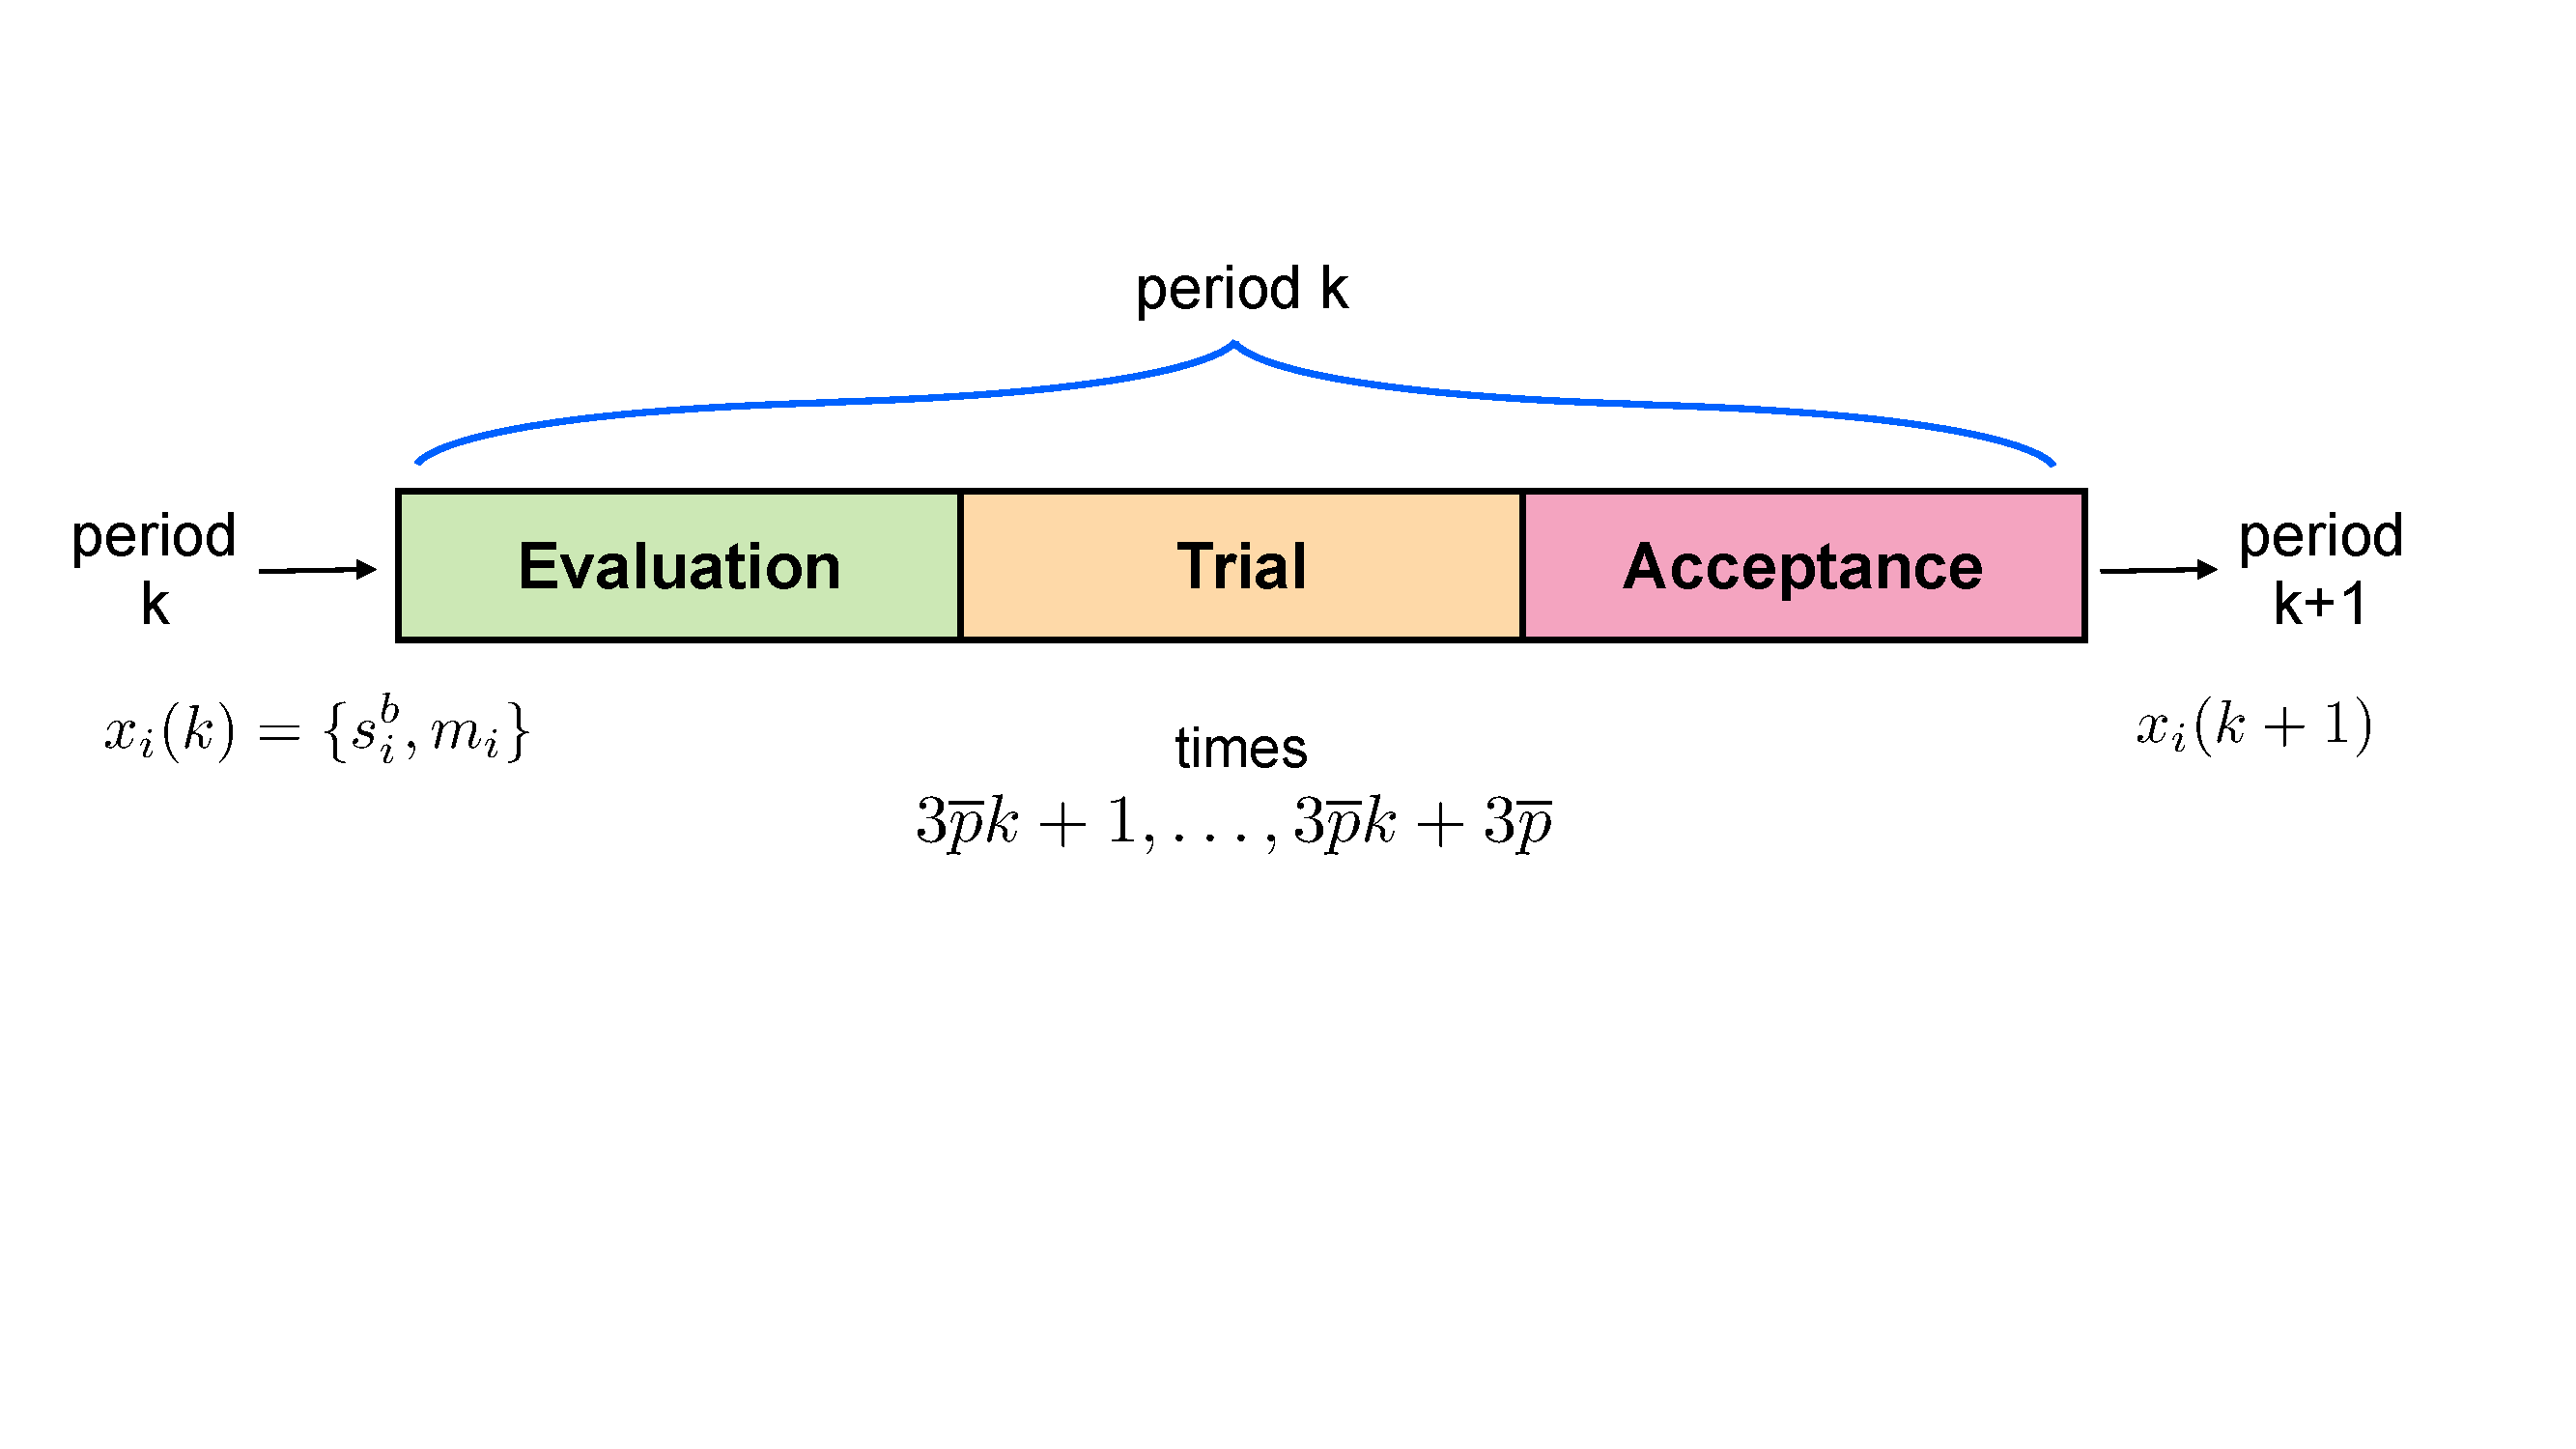
\includegraphics[trim = 0mm 100mm 20mm 40mm, clip, width=\columnwidth]{algorithm.pdf}
\caption{Learning algorithm phases within each time period}
\end{center}
\end{figure}
%
The times $\{1, 2, \dots\}$ will be broken up into periods of length $3 \bar{p}$ where $\bar{p} > 1$ is an interval whose length will be defined formally below.  At the beginning of each period $k$, each agent $i \in N$ has a local state variable of the form $x_i(k) = [s_i^b, m_i]$ where $s_i^b \in S_i$ is the agent's baseline strategy and $m_i$ is the agent's mood.  The agent's baseline strategy corresponds to the strategy the agent is accustomed to playing.  The agent's mood $m_i$, which can either be \textsc{Content} or \textsc{Discontent}, dictates how likely each agent is to select its baseline strategy during a given period.  Roughly speaking, a content agent is more likely to select its baseline strategy while a discontent agent is more likely to try an alternate strategy.  

Each period $k > 0$, which consists of the time steps $\{3 \bar{p} k + 1, \dots, 3 \bar{p} (k + 1)\}$, will be broken up into three distinct phases called {\it evaluation}, {\it trial}, and {\it acceptance}.  The behavior of the agents in each of these phases is highlighted below:
%

\vspace{.1cm}
%
\noindent -- {\it Evaluation Phase:} The first phase is the {\it evaluation phase}. In this phase, each agent  establishes a baseline utility, $u_i^b$, associated with its current baseline strategy, $s_i^b.$ All agents commit to their baseline strategies during this entire phase.

\vspace{.1cm}
%
\noindent -- {\it Trial Phase:} The second phase is the {\it trial phase}. During this phase, each agent has the opportunity to experiment with an alternate trial strategy, $s_i^t,$ in order to determine whether changing its baseline strategy could be advantageous. An agent's mood determines how likely it is to experiment.  In particular, a content agent will use its baseline strategy $s_i^b$ during the trial phase with high probability.  On the other hand, a discontent player is likely to experiment with a trial strategy $s_i^t \neq s_i^b$.  The exact probabilities associated with this selection process will be described in detail in the forthcoming section.   

\vspace{.1cm}
%
\noindent -- {\it Acceptance Phase:} The third phase is the {\it acceptance phase}. Here, an agent who experimented during the trial phase decides whether to accept its trial strategy or revert to its baseline strategy. Agents who did not experiment during the trial phase commit to their baseline strategies and observe payoff changes which occur due to others' changes in strategy.  


\subsection{Formal algorithm description}\label{s:algorithm}


We begin by defining a constant $c > n$, an experimentation rate $\eps\in (0,1)$, and the length of a phase to be $\p = \lceil 1/\delta^{nc+1}\rceil$ time steps, for some small $\delta\in (0,1)$. A period consists of the evaluation, trial, and acceptance phases, and hence is $3\bar{p}$ time steps long. Let $x_i = x_i(k) = [s_i^b, m_i]$ represent that state of each agent $i \in N$ at the beginning of some period $k \in \{1, 2, \dots\}$.  We will formally present the algorithm using the same general structure given in previous section.  

\vspace{.2cm}

\noindent {\textbf{Agent Dynamics:}}  Here we describe how individual agents make decisions within a given period.  Decisions of an agent $i \in N$ are influenced purely by its state at the beginning of the $k$-th period, $x_i(k)$, and by payoffs received during the $k$-th period.  We specify agents' behavior during the $k$-th period for the three phases highlighted above.   



\vspace{.2cm}
%
\noindent {\it \textbf{-- Evaluation Phase:}} The evaluation phase consists of the times $t \in \{3\p k + 1, \dots, 3\p k+\p\}$.  Throughout this phase, each agent commits to its baseline strategy $s_i^b$.  At the end of the phase, each agent computes its average baseline utility, 
%
\begin{equation}\label{e:baseline payoff}
u_i^b = {1\over \p}\sum_{\tau = 3 \p k+1}^{3\p k+\p}U_i\bigl(\s_1^b(z(\tau), \dots, \s_n^b(z(\tau))  \bigr),
\end{equation}
%
where $z(\tau)$ denotes the common random signal observed at time $\tau$.  Here, $u_i^b$ is viewed as an assessment of the performance associated with the baseline strategy $s_i^b$.  


\vspace{.1cm}
%
\noindent {\it \textbf{-- Trial Phase:}} After the evaluation phase comes the trial phase which consists of the times $t \in \{(3\p k + \p)+1,\ldots ,3\p k +2 \p\}$.  During the trial phase each player $i\in N$ may try a strategy other than its baseline, and must commit to this trial strategy, $s_i^t \in S_i$, over the entire phase.  Agents' trial strategies are selected according to the following rule:
%


\begin{itemize}%[leftmargin = .3cm]
%{\setlength\leftmargin{0in}}
%
\item {\it Content, $m_i = C$:}
When agent $i$ is content, its trial strategy, $s_i^t \in S_i$, is chosen according to the  distribution
\begin{equation}
\Pr\left[s_i^t = s_i \right] = \left\{
\begin{array}{ll}
1 - \eps^c &\text{if }s_i = s_i^b \\
\eps^c \mathbin{/} |\mathcal{A}_i|&\text{for any } s_i = a_i\in\mathcal{A}_i
\end{array}\right.
\end{equation}
%
A strategy $s_i^t = a_i$ means that agent $i$ commits to playing action $a_i$ for the entire trial phase of the $k$-th period, i.e., the strategy does not depend on the common random signal.  Observe that a content player predominantly selects its baseline strategy during the trial phase.

\item {\it Discontent, $m_i = D$:}
When agent $i$ is discontent, its trial strategy, $s_i^t$, is chosen randomly from the set $S_i$,
\begin{equation}\label{eq:981}
\Pr\left[s_i^t = s_i\right] = 1\mathbin{/} |S_i| \text{ for all } s_i\in S_i.
\end{equation}
%
%\vspace{.1cm}

%
\end{itemize}

At the end of the trial phase, each agent computes its average utility:
%
\begin{equation}\label{e:trial payoff}
u_i^t = {1\over \p}\sum_{\tau = 3\p k + \p)+1}^{3\p k +2 \p}U_i\bigl(\s_1^t(z(\tau), \dots, \s_n^t(z(\tau))  \bigr).
\end{equation}
%
Here, $u_i^t$ is viewed as an assessment of the performance associated with the baseline strategy $s_i^t$.  
%

%
\noindent {\it \textbf{-- Acceptance Phase:}} The last phase is the acceptance phase which consists of times $t \in \{(3 \p k + 2\p)+1, \dots, 3\p k + 3\p\}$.  The primary purpose of the acceptance phase is to further evaluate changes in the payoffs between $u_i^b$ and $u_i^t$.  Each agent $i \in N$ commits to an acceptance strategy, denoted by $s_i^a \in S_i$, over the entire acceptance phase.  Each agent's acceptance strategy is selected according to the following.
%

\begin{itemize}%[leftmargin = .3cm]
%
\item {\it Content, $m_i = C$:}
When agent $i$ is content, its acceptance strategy is chosen as follows:
\begin{equation}
s_i^a = \left\{
\begin{array}{ll}
s_i^t &\text{if } u_i^t > u_i^b + \delta, \\
s_i^b &\text{if } u_i^t \leq u_i^b + \delta. 
\end{array}\right.
\end{equation}
%
That is, players only repeat their trial strategy if their performance was high enough relative to the performance of the baseline strategy.  

\item {\it Discontent, $m_i = D$:}
When agent $i$ is discontent, the acceptance strategy is set as $s_i^a = s_i^t$.
\end{itemize}

Following the acceptance phase, each agent computes its average utility:
%
\begin{equation}\label{e:acceptance payoff}
u_i^a = {1\over \p}\sum_{\tau = (3 \p k + 2\p)+1}^{3\p k + 3\p}U_i\bigl(\s_1^a(z(\tau), \dots, \s_n^a(z(\tau))  \bigr).
\end{equation}
%
Here, $u_i^a$ is viewed as an assessment of the performance associated with the baseline strategy $s_i^a$.  
%
%


\vspace{.2cm}

\noindent {\textbf{State Dynamics:}}  After the agent dynamics comes the state dynamics which specifies how the state of each agent evolves.  The state of each agent $i \in N$ at the beginning of the $k+1$-st stage, i.e., $x_i(k+1)$, is influenced purely its state at the beginning of the $k$-th period, i.e., $x_i(k)$, the strategies $s_i^b,$ $s_i^t$ and $s_i^a$, and the payoffs received during the $k$-th period.   The state dynamics are broken into the following cases:
%  

\vspace{.2cm}

%
\noindent {\it {-- Content and No Experimentation, $m_i = C, s_i^t = s_i^b$:}} 
%
If agent $i$ was content at the start of the $k$-th period and did not experiment in the trial phase, its state at the beginning of the $(k+1)$-st period is chosen as follows:
\begin{itemize}% [leftmargin = .3cm]
\item If $u_i^a \geq u_i^b - \delta,$
\begin{equation}\label{e:state trans1a}
x_i(k+1) = \left\{
\begin{array}{ll}
\left[s_i^a = s_i^b,\, C\right] &\quad\text{w.p. }1-\eps^{2c}, \\
\left[s_i^a = s_i^b,\, D\right] &\quad\text{w.p. } \eps^{2c}.
\end{array}\right.
\end{equation}
\item If $u_i^a < u_i^b - \delta$,
\begin{equation}\label{e:state trans1b}
x_i(k+1) = 
\left[s_i^a = s_i^b,\, D\right] 
\end{equation}
\end{itemize}
%
Accordingly, if the agent's average payoff during the acceptance phase is low enough, then it will become discontent.  

\vspace{.1cm}

%
\noindent {\it {-- Content and Experimentation, $m_i = C, s_i^t \neq s_i^b$:}} 
%
If agent $i$ was content at the start of the $k$-th period and experimented during the trial phase, its state at the beginning of the $(k+1)$-st period is chosen as 
\begin{equation}\label{e:state trans2}
x_i(k+1) = \left[s_i^a, C\right].
\end{equation}
%
In this case the agent's average payoff during the acceptance phase does not impact its underlying state dynamics.  

\vspace{.1cm}

%
\noindent {\it {-- Discontent, $m_i = D$:}} 
%
If agent $i$ was discontent at the start of the $k$-th period, its state at the beginning of the $(k+1)$-th period is chosen as follows
%
\begin{equation}\label{e:D state trans}
x_i(k+1) = \left\{
\begin{array}{ll}
\left[s_i^a, C\right] &\text{w.p. }  \eps^{1-u_i^a}, \\
\left[s_i^a, D\right] &\text{w.p. } 1 - \eps^{1-u_i^a}. 
\end{array}\right.
\end{equation}
%
Here, the agents are more likely to become content with strategies the yield higher average payoffs. 


\section{Main Result}

Throughout this chapter we focus on games where there is some degree of coupling between the utility functions of the agents.  The following definition of interdependence, taken from \cite{Young2009}, captures this notion of coupling.  
 
\begin{defn}
A game $G$ with agents $N = \{1,2,\ldots,n\}$ is said to be {\it interdependent} if, for every $a\in\mathcal{A}$ and every proper subset of agents $J\subset N$, there exists an agent $i\notin J$ and a choice of actions $a_J^\prime\in\prod_{j\in J} \mathcal{A}_j$ such that $U_i(a_J^\prime,a_{-J})\neq U_i(a_J,a_{-J}).$
\end{defn}

Roughly speaking, the definition of interdependence states that it is not possibly to partition the group of agents into two sets whose actions do not impact one another's payoffs.

The following theorem characterizes the limiting behavior associated with the proposed algorithm. 

\secondtheorem*
%\begin{Theorem}\label{t:main theorem CCE}
%
%Let $G = \left (N,\{U_i\},\{\mathcal{A}_i\}\right)$ be a finite interdependent game. 
%
%First, suppose $q(S) \cap {\rm CCE} \neq \emptyset$.  Given any probability $p < 1$, if the exploration rate $\eps$ is sufficiently small, and if $\delta = \eps$, then for all sufficiently large times $t$,\footnote{For the proof of Theorem~\ref{t:main theorem CCE}, we require $\delta = \eps$. However, in practice, fixing $\delta>\eps$ in order to shorten the period length, $\bar{p},$ often yields similar results, as we demonstrate in Example~\ref{e:example}.}
%
%$$ {\rm Pr} \left[q(s(t)) \in \underset{ q \in q(S) \cap {\rm CCE}}{\arg \max} \ \sum_{i \in N} \sum_{a \in \aee} \ U_i(a) q^a \right] > p. $$ 
%
%Alternatively, suppose $q(S) \cap {\rm CCE} = \emptyset$.  Given any probability $p < 1$, if the exploration rate $\eps$ is sufficiently small and $\delta = \eps$, then for all sufficiently large times $t$, 
%
%$$ {\rm Pr} \left[q(s(t)) \in \underset{ q \in q(S)}{\arg \max} \ \sum_{i \in N} \sum_{a \in \aee} \ U_i(a) q^a \right] > p. $$ 
%
%\end{Theorem}

\vspace{.1cm}

We prove Theorem~\ref{t:main theorem CCE} in Appendix~\ref{s:proof CCE}.

A few remarks are on order regarding Theorem~\ref{t:main theorem CCE}.  First, observe that the proposed algorithm is of the form (\ref{eq:2321}).  Second, the condition $q(S) \cap {\rm CCE} \neq \emptyset$ implies the agents can realize specific joint distributions that are coarse correlated equilibria through the joint strategy set $S$.  When this is the case, the above algorithm ensures the agents predominantly play a strategy $s \in S$ where the resulting joint distribution $q(s)$ corresponds to the efficient coarse correlated equilibrium.  Alternately, the condition $q(S) \cap {\rm CCE} = \emptyset$ implies there are no agent strategies that can characterize a coarse correlated equilibrium.  When that is the case, the above algorithm  ensures the agents predominantly play strategies that have full support on the action profiles $a \in \aee$ that maximize the sum of the agents payoffs, i.e., $\arg \max_{a \in \aee} \sum_{i \in N} U_i(a)$.

\section{Illustrative Example}\label{s:example}

Here, we present an example where agents update their strategies according to the algorithm above, and their actions converge to an efficient coarse correlated equilibrium.

\begin{example}\label{e:example}
Consider a game with two players, (Row, Column), and the following payoff matrix:
\begin{center}
\begin{tabular}{c|c|c|c|}
\multicolumn{1}{r}{}&
	\multicolumn{1}{c}{{L}}&
		\multicolumn{1}{c}{{M}}&
			\multicolumn{1}{c}{{R}}\\
\cline{2-4}T &0, 0&0, 1&0.85, 0.75\\
\cline{2-4}{M}&1, 0&0, 0&0, 0\\
\cline{2-4}{B}&0.75, 0.85&0, 0&0, 0\\\cline{2-4}
\end{tabular}
\end{center}

\smallskip

The efficient coarse correlated equilibrium in this game places probability 0.5 on joint action (T,R), and probability 0.5 on joint action (B,L), i.e., 
\begin{equation}\label{e:efficient CCE}
q^{(T,R)} = q^{(B,L)} = 0.5,
\end{equation}
and $q^a = 0$ for $a\notin\{(T,R), (B,L)\}.$ The expected utility associated with this coarse correlated equilibrium is 
$U_i(q) = 0.8.$

For each value of $\eps$ in $\{0.15, 0.1, 0.015,0.01\}$, we simulated our algorithm for 20 times over $10^5$ iterations, fixing $\delta = 0.14$. The table below shows the percentage of the last $5\times 10^4$ iterations spent in the efficient coarse correlated equilibrium as in \eqref{e:efficient CCE}.\footnote{We did not simulate our algorithm for smaller values of $\eps$ because convergence rates slow significantly as $\eps\to 0,$ reducing the algorithm's practicality. Next research steps include improving this algorithm's convergence rates. }

\begin{table}[H]
%\caption{default}
\begin{center}
\begin{tabular}{|c|c|}\hline
$\m{\eps}$ 	& \tb{\% time in efficient CCE}	\\\hline\hline
0.15 			& 9\%					\\\hline
0.1 			&16\%					\\\hline
0.015			&84\%					\\\hline
0.01			&87\%\\\hline
\end{tabular}
\end{center}
%\label{default}
\end{table}%

Note that as $\eps$ decreases, more time is spent in the efficient coarse correlated equilibrium, as predicted by Theorem~\ref{t:main theorem CCE}.


%We note that, although Theorem~\ref{t:main theorem} requires $\delta = \eps$, setting $\delta$ significantly larger in practice appears to yield similar long term behavior, as shown in this example.

%\red{FINISH THIS EXAMPLE}


\end{example}


%\section{Conclusion}

The majority of distributed learning literature has focused on identifying learning rules that converge to Nash equilibria.  However, alternate forms of behavior, such as correlated equilibrium, can often lead to significant improvements in system-wide behavior.  This chapter focuses on identifying learning rules that converge to joint distributions that do not necessarily constitute Nash equilibria.  In particular, we have a provided a distributed learning rule, similar in spirit to the learning rule in \cite{Marden2013c}, that ensuers agents play strategies that constitute efficient coarse correlated equilibria. A mild variant of the proposed algorithm could also ensure the agents play strategies that constitute correlated equilibria, as opposed to coarse correlated equilibria.  Future work seeks to investigate the applicability of such algorithms in the context of team versus team zero-sum games.  